\documentclass[a4paper,11pt]{article}
  
\usepackage{graphicx}
\usepackage{amsmath}
\usepackage{array}
\usepackage{float}
\usepackage{subfigure}
\usepackage{color}
\usepackage{listings}
\usepackage[utf8x]{inputenc}
\usepackage{hyperref}
\usepackage{rotating}

\usepackage{amsfonts}  % For \mathbb

% Read MRPT version:
\newread\file
\openin\file=../../version_prefix.txt
\read\file to\MRPTVERSION % Reads a line of the file 
\closein\file

% Title Page
\title{User guide for \texttt{libmrpt-srba}: A generic C++ framework for Relative Bundle Adjustment (RBA)}
\author{Jose-Luis Blanco-Claraco \\ joseluisblancoc@gmail.com \\ \texttt{http://www.mrpt.org/} }
\date{MRPT version: \MRPTVERSION \\ Document build: \today }

% C++ listings settings
\lstset{ %
language=C++,                % choose the language of the code
basicstyle=\footnotesize,       % the size of the fonts that are used for the code
numbers=none,                   % where to put the line-numbers
numberstyle=\footnotesize,      % the size of the fonts that are used for the line-numbers
stepnumber=1,                   % the step between two line-numbers. If it is 1 each line will be numbered
numbersep=5pt,                  % how far the line-numbers are from the code
backgroundcolor=\color{white},  % choose the background color. You must add \usepackage{color}
commentstyle=\color{blue},
showspaces=false,               % show spaces adding particular underscores
showstringspaces=false,         % underline spaces within strings
showtabs=false,                 % show tabs within strings adding particular underscores
frame=single,           % adds a frame around the code
tabsize=2,          % sets default tabsize to 2 spaces
captionpos=b,           % sets the caption-position to bottom
breaklines=true,        % sets automatic line breaking
breakatwhitespace=false,    % sets if automatic breaks should only happen at whitespace
escapeinside={\%*}{*)}          % if you want to add a comment within your code
}

\begin{document}
\maketitle


\vfill

\begin{scriptsize}
\begin{center}
\includegraphics[width=3cm]{imgs/by-nc-nd-eu.pdf}
\\
This work is licensed under a Creative Commons Attribution-NonCommercial-NoDerivs 3.0 Unported License.
\end{center}
\end{scriptsize}

\vspace{1cm}

\newpage

\textbf{Revision history:}
\begin{itemize}
 \item Feb 2013: First version. Released along MRPT 1.0.0.
\end{itemize}

\vfill


\begin{small}
In case you want to cite this guide in your academic publications, here is a BibTeX entry: 

\begin{verbatim}
@MISC{libmrpt-srba-guide,
  author = {Jose-Luis Blanco-Claraco},
  title = {{User guide for \texttt{libmrpt-srba}: A generic 
      C++ framework for Relative Bundle Adjustment (RBA)}},
  howpublished = {http://www.mrpt.org/srba},
  year = {2013}
} 
\end{verbatim} 

\end{small}

\vspace{1cm}

\newpage
\tableofcontents
\newpage

\section{Introduction}

Bundle adjustment (BA) is the name given to one solution to visual SLAM based on maximum-likelihood estimation (MLE) 
over the space of map features and camera poses. However, it is by no way limited to visual maps, since the same 
optimization techniques employed in BA are also applicable to maps of pose constraints (graph-SLAM) and to many other 
kind of feature maps, not necessarily involving visual information.

The framework of \emph{Relative Bundle Adjustment (RBA)} was introduced in a series of works by Gabe Sibley and 
colleagues in \cite{sibley2009rba,sibley2009adaptive}. 

\emph{Sparser RBA (SRBA)} is the name of the generic and extensible framework for RBA, implemented in 
the C++ library \texttt{mrpt-srba}. It features the introduction of 
a \emph{constant-time algorithm} for maintaining problem graphs with arbitrary topologies 
(as presented in \cite{blanco2013srba}), as well as a generic design which allows turning RBA 
into \emph{relative Graph-SLAM} (i.e. networks of relative pose constraints whose solution are also relative poses).

\section{Library installation}

\texttt{mrpt-srba} is one of the libraries of the Mobile Robot Programming Toolkit (MRPT). 
It is header-only and makes \emph{intensive} use of templates and design patterns for the sake of customization, 
flexibility and extensibility. 

Note however that it depends on other non-header-only libraries\footnote{The link-time dependencies are: \texttt{mrpt-base} 
for geometry, math auxiliary classes, serialization,... and \texttt{mrpt-opengl} for generating 3D representations of 
the RBA problems. Despite its name, the latter library can be built for platforms without any 
functional \texttt{OpenGL} implementation, though it is recommended to always visualize the results for getting a better 
insight of what is going on in your programs. The header-only library \texttt{Eigen} \cite{eigenweb} is also a mandatory dependency, but 
an embedded version is shipped with \texttt{mrpt-base} in case the user does not have it installed.}, 
so in practice before using \texttt{mrpt-srba} in your program you need
both (i) access to headers (\texttt{.h} files) and (ii) binary libraries to link against them. 

In Ubuntu, installing the package \texttt{libmrpt-dev} (version 1.0.0 or newer) is the easiest way to have 
everything ready to start coding your own programs. You can also install \texttt{mrpt-apps} for the application \texttt{srba-slam} 
and a set of sample datasets (see \S\ref{sect:srba_slam_app}).

If your official repository has an older version of the package, use this PPA repository instead:

\begin{lstlisting}
 sudo add-apt-repository ppa:joseluisblancoc/mrpt
 sudo apt-get update
 sudo apt-get install libmrpt-dev mrpt-apps
\end{lstlisting}

Binary packages for Windows are also available online\footnote{\href{http://www.mrpt.org/download}{http://www.mrpt.org/download}}.
If you prefer to build MRPT from sources, please visit the official web\footnote{\href{http://www.mrpt.org/}{http://www.mrpt.org/}} 
for detailed instructions.


\section{RBA primer}
\label{sect:rba_primer}

This manual will not explain the mathematical details of how RBA is modeled and solved -- please, refer to cited papers.
Though, it is mandatory to clearly establish which \textbf{entities} define an RBA problem before discussing the library API.

An example such that the one in Fig.~\ref{fig:rba.entities} will help introducing the different elements.
The illustration depicts many elements, some of which are \emph{known} data, others are the problem \emph{unknowns}. 
The goal of RBA is to recover a \emph{maximum-likelihood estimation (MLE)} of those unknowns. Optionally, the covariances and 
cross-covariances between estimated variables can be also evaluated.

\begin{figure}[h]
\centering
%\includegraphics[width=1.0\textwidth]{imgs/rba-entities.pdf} 
\caption{A toy RBA problem.}
\label{fig:rba.entities}
\end{figure}

We find the following entities in \texttt{mrpt-srba}:

\begin{itemize}
\item{\textbf{Keyframes}: A keyframe (KF) represents the \emph{pose} of the robot (or any device of interest) at one 
 particular instant of time. In RBA we will never work with the absolute coordinates of any of these KFs. This is 
 completely different than ``common'' Bundle Adjustment, where these poses are the unknowns to estimated  
 complete 
}
\end{itemize}




\section{Programmer's first steps}
\label{sect:program_first}

\subsection{First program}

\begin{lstlisting}
void main()
{
	// Code 
    int a; /* pepe */
}
\end{lstlisting}

\subsection{Tutorials}

An example screenshot is shown in Fig.~\ref{fig:screenshot.tutorial1}.

\begin{figure}
\centering
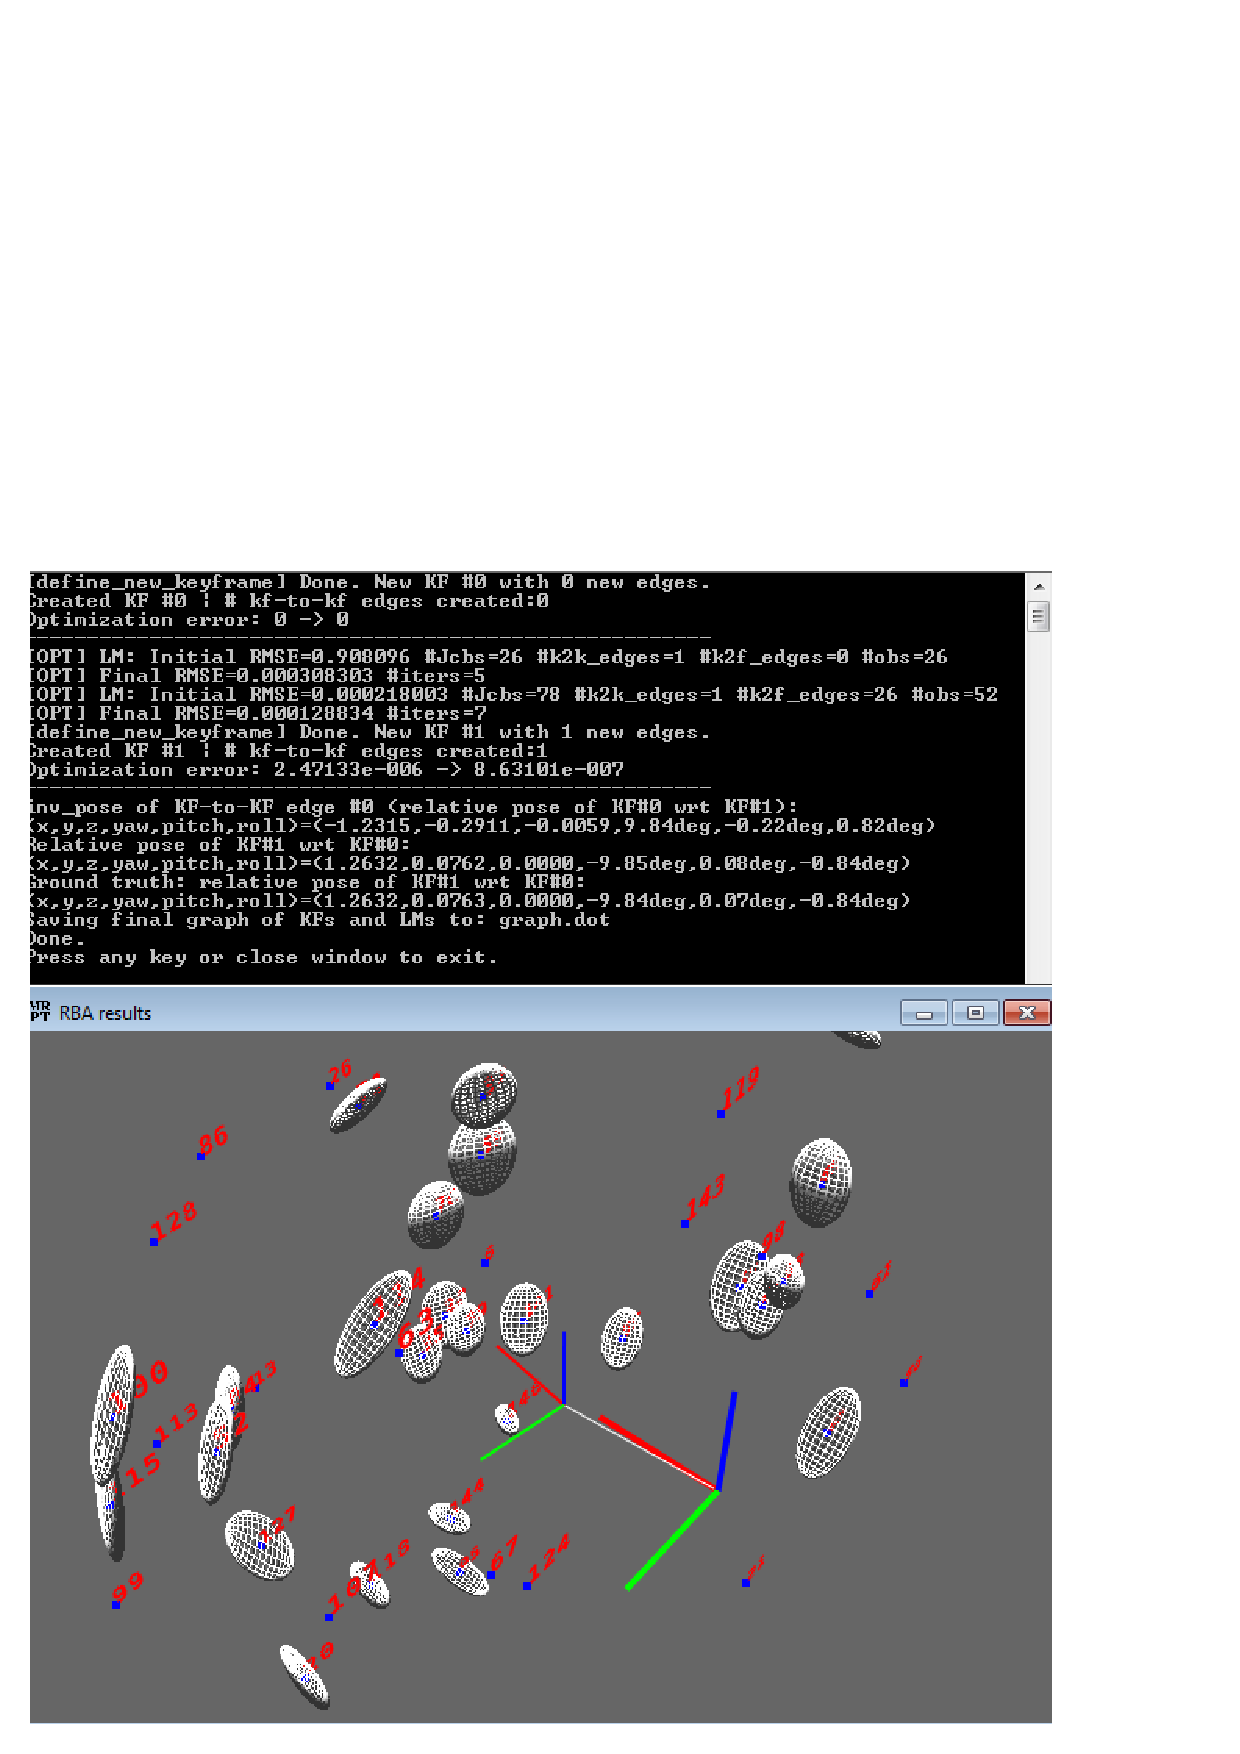
\includegraphics[width=1.0\textwidth]{imgs/screenshot_tutorial_range-bearing-3D.pdf} 
\caption{Screenshot for \texttt{tutorial-srba-range-bearing-se3.cpp}.}
\label{fig:screenshot.tutorial1}
\end{figure}


\section{Existing models}
\label{sect:program_models}

\subsection{KF-to-KF relative poses}

XXXX XXXX 

\subsection{Relative landmark parameterizations}

XXXX XXXX 

\subsection{Observation types}

XXXX XXXX 


\section{Sensor models}
\label{sect:program_sensors}

XXXX XXXX 


\section{The \texttt{srba-slam} application}
\label{sect:srba_slam_app}

XXXX


\section{Library inner structure}

\subsection{Directory layout}


\subsection{Data structures}


\begin{sidewaysfigure}
\centering
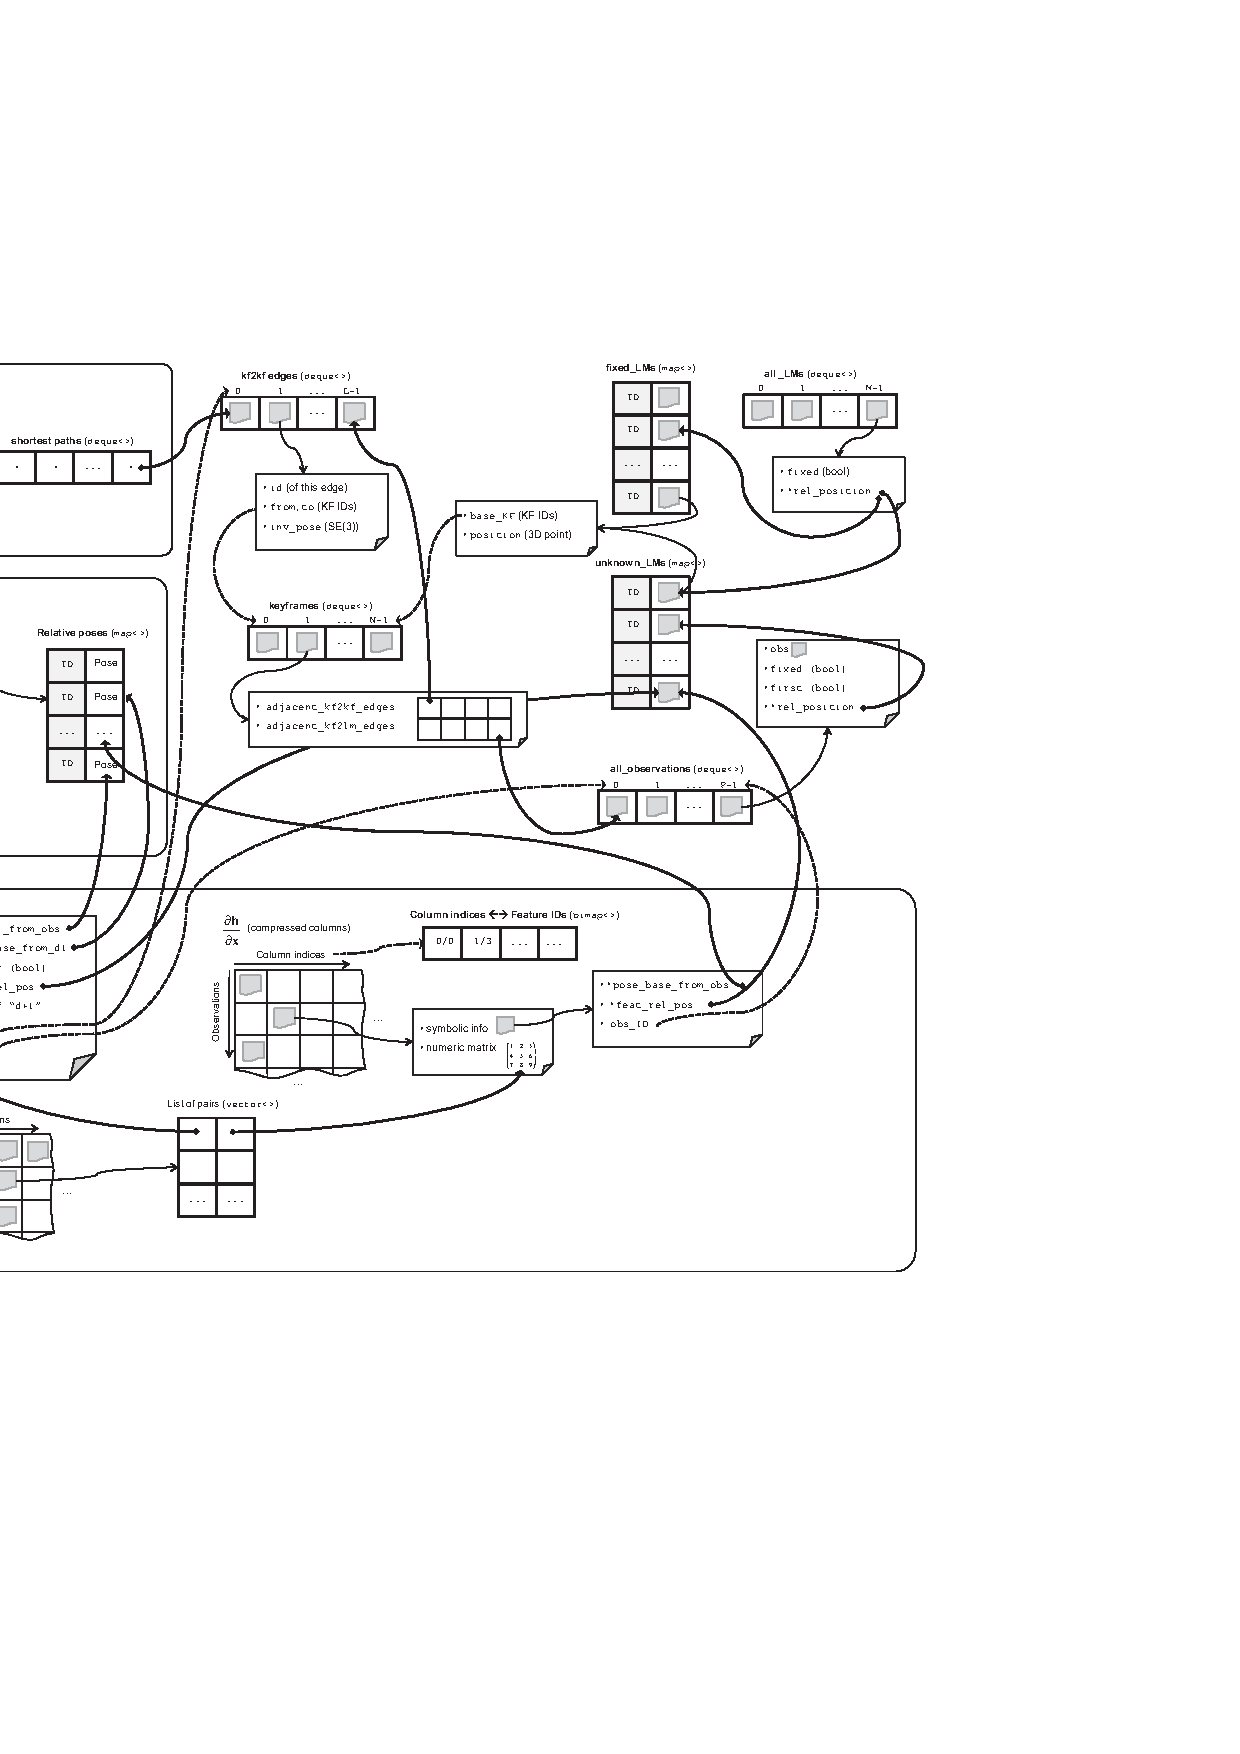
\includegraphics[width=1.0\textwidth]{imgs/srba_data_structures.pdf} 
\caption{Detailed data structures. Refer to the legend for the format of structures and pointers/references.}
\label{fig:detailed.data.structures}
\end{sidewaysfigure}





%% ---------------------------------------------------------------
%%                         BIBLIOGRAPHY
%% ---------------------------------------------------------------
\newpage
\bibliographystyle{plain}
\bibliography{cites}

\end{document}

